\chapter{Literature Review\label{chap:litreview}}

This chapter situates \textsc{SciFig-Eval} against six strands of prior art: chart benchmarks (\S\ref{sec:lit-benchmarks}), hallucination and visual shortcuts (\S\ref{sec:lit-halluc}), robustness and misleading visualisations (\S\ref{sec:lit-robust}), multilingual figure understanding (\S\ref{sec:lit-multiling}), behavioural evaluation of honesty, sycophancy and induction (\S\ref{sec:lit-behave}), and the evaluation of evaluators (\S\ref{sec:lit-eval-of-eval}).
Each section closes with the specific gap that \textsc{SciFig-Eval} addresses; \S\ref{sec:lit-synthesis} synthesises the diagnosis and positions the present work.

\section{Chart and Scientific-Figure Benchmarks}
\label{sec:lit-benchmarks}

The chart-understanding benchmark literature has arrived in three
waves. The earliest, clustered around 2018--2020, is
\emph{synthetic}. FigureQA \citep{kahou2018figureqa} and PlotQA
\citep{methani2020plotqa} generate plots programmatically and ask
templated questions about structure, retrieval and numerical
reasoning. Their scale is impressive, with PlotQA alone offering
close to 29~million question--answer pairs, but their visual
diversity is narrow, and models trained on them transfer poorly to
real publication figures.

A second wave, beginning with ChartQA \citep{masry2022chartqa} and
extended by Chart-to-Text \citep{kantharaj2022charttotext}, moves to
real charts curated from Statista, Pew Research and similar sources,
and it broadens the task inventory from closed QA to summarisation.
ChartQA's \emph{Relaxed Accuracy} metric, which tolerates small
numerical error on open-string answers, set the de facto standard
for chart QA, while Chart-to-Text noted early that fluency on chart
captions and faithfulness to the chart come apart routinely. The
same observation recurs, in stronger form, in CHOCOLATE
\citep{huang2024chocolate}, which analyses factual errors in
LVLM-generated chart captions and finds them structured enough to
type.

The third wave, 2024--2025, pushes into genuine scientific
publication figures and genuine reasoning. CharXiv
\citep{wang2024charxiv} hand-curates 2{,}323 charts from arXiv and
reports that frontier models reach roughly 80\% on descriptive items
yet only 47\% on reasoning, while expert humans remain near 80\% on
the latter. SciFIBench \citep{huang2024scifibench} and ChartQAPro
\citep{masry2025chartqapro} sharpen different edges of the same
blade. The former targets publication-quality figure interpretation,
while the latter introduces unanswerable and conversational items
that break saturation on easier chart benchmarks. ChartMuseum
\citep{tang2025chartmuseum} labels questions by reasoning type and
exposes a large gap between \emph{text-primary} items, on which
models look competent, and \emph{visual-primary} items, on which
they collapse. MultiChartQA \citep{zhu2024multichartqa} adds a
compositional axis, requiring cross-chart integration that
single-chart benchmarks cannot capture.

\begin{table}[t]
  \centering
  \footnotesize
  \setlength{\tabcolsep}{3.5pt}
  \renewcommand{\arraystretch}{1.18}
  \caption[Representative chart and scientific-figure benchmarks.]{%
    Representative chart and scientific-figure benchmarks in
    chronological order. \emph{Task} abbreviations cover QA
    (short-answer question answering), Cap (caption generation),
    D$+$R (descriptive and reasoning items scored separately),
    V/T (visual-primary versus text-primary items) and Desc
    (paragraph-length description). The \emph{Open} column flags
    benchmarks whose primary task admits open-ended,
    paragraph-length generation. The \emph{Reasoning} column flags
    benchmarks that separate reasoning from description, and the
    \emph{Behav.} column flags benchmarks that probe
    behavioural axes such as honesty, abstention or robustness
    ($\checkmark$ full, $\circ$ partial, -- not supported).
    \textsc{SciFig-Eval} occupies the intersection that the
    earlier waves leave unfilled.}
  \label{tab:lit-benchmarks}
  \begin{tabular}{@{}l c l l l c c c@{}}
    \toprule
    \textbf{Benchmark} & \textbf{Year} & \textbf{Source} &
    \textbf{Languages} & \textbf{Task} & \textbf{Open} &
    \textbf{Reas.} & \textbf{Behav.} \\
    \midrule
    FigureQA      & 2018 & Synthetic    & EN        & QA              & --         & --         & --         \\
    PlotQA        & 2020 & Synthetic    & EN        & QA              & --         & --         & --         \\
    ChartQA       & 2022 & Web          & EN        & QA              & --         & $\circ$    & --         \\
    Chart-to-Text & 2022 & Web          & EN        & Cap             & \checkmark & --         & --         \\
    CharXiv       & 2024 & arXiv        & EN        & QA (D$+$R)      & --         & \checkmark & --         \\
    SciFIBench    & 2024 & Scientific   & EN        & QA              & --         & $\circ$    & --         \\
    MultiChartQA  & 2024 & Real (web)   & EN        & Multi-chart QA  & --         & \checkmark & --         \\
    ChartMuseum   & 2025 & Real (web)   & EN        & QA (V/T)        & --         & \checkmark & --         \\
    ChartQAPro    & 2025 & Web $+$ news & EN        & QA (conv./unans.)& $\circ$   & \checkmark & $\circ$    \\
    PolyChartQA   & 2025 & Re-rendered  & EN $+$ 9  & QA              & --         & $\circ$    & --         \\
    \midrule
    \rowcolor{black!7}
    \textbf{\textsc{SciFig-Eval}} & \textbf{2026} &
    \textbf{Native venues} & \textbf{EN/BG/DE/ZH} &
    \textbf{Desc.\ $+$ probes} & \textbf{\checkmark} &
    \textbf{\checkmark} & \textbf{\checkmark} \\
    \bottomrule
  \end{tabular}
\end{table}

Three properties characterise this benchmark literature in
aggregate. First, it is overwhelmingly short-form. Systematic
evaluation of open-ended, paragraph-length descriptions of real
scientific figures remains thin, with Chart-to-Text and CHOCOLATE
the main exceptions. Second, it is overwhelmingly English. Only a
handful of the benchmarks cited above include non-English splits,
and none cover typologically diverse scientific figures at
publication quality. Third, reasoning questions rarely separate
``reasoning the figure compels'' from ``reasoning the caption
invites'', a distinction the next section will show to be central.
\textsc{SciFig-Eval} extends this strand along the three axes on
which it is thinnest, namely open-ended, multilingual,
reasoning-aware description of real publication figures, scored
through typed error dimensions rather than exact match.

\section{Hallucination, Visual Shortcuts, and the Vision--Language Bottleneck}
\label{sec:lit-halluc}

Hallucination on chart-like inputs has been documented along three
complementary lines of attack. The first treats hallucination
taxonomically. ChartHal \citep{xu2025charthal} organises fine-grained
hallucination on chart QA into irrelevant, non-existent and
contradictory scenarios and shows that strong models remain poor
once each scenario is scored separately. CHOCOLATE
\citep{huang2024chocolate} performs the equivalent exercise on chart
\emph{captioning} and finds that fluent captions systematically
smuggle in factual errors. HallusionBench
\citep{guan2024hallusionbench} further decomposes hallucination into
two distinct failure modes. The first, \emph{language hallucination},
occurs when the decoder over-generates beyond what vision supports.
The second, \emph{visual illusion}, occurs when the encoder
misperceives. HallusionBench argues that treating the two jointly
has obscured both.

The second line asks whether the image matters at all.
\citet{li2025seeorrecall} run a striking diagnostic. On popular
visualisation-QA benchmarks, many items can be solved at
frontier-model accuracy \emph{without showing the image}, because
either question context or option structure leaks the answer. The
implication is that much of what is reported as multimodal
competence is in fact parametric recall from the language side. ARO
\citep{yuksekgonul2022aro} shows, in parallel, that several
vision--language models behave like bags of words on captioned
images, under-using order and relational structure in ways consistent
with a textual rather than visual solution. ChartMuseum's
\citep{tang2025chartmuseum} sharp gap between text-primary and
visual-primary items, at similar aggregate difficulty, is the same
phenomenon from the evaluation side, in that apparent chart
competence often reflects reading chart \emph{text} rather than
reading chart \emph{graphics}.

The third line attempts a shallow mechanistic account. FUGU
\citep{tartaglini2025fugu} runs controlled scatter-plot interventions
on three vision--language models and argues that a major bottleneck
sits at the vision--language hand-off. Correct coordinates can be
probed out of the vision tower while the final answer is wrong, and
supplying oracle coordinates helps single-point tasks yet sometimes
hurts aggregate ones. Fine-tuning alone does not reach ceiling,
which points to a residual architectural limit rather than a
data-coverage issue.

These three lines jointly explain why purely accuracy-based
benchmarks flatter models. The language decoder can manufacture
plausible output, the evaluation protocol can reward it, and the
image itself is often redundant to the extent that text context
leaks. \textsc{SciFig-Eval} inherits the ChartHal and CHOCOLATE
error typology but applies it to \emph{open-ended descriptions} of
real scientific figures in four languages, and it builds explicit
probes, including a selective-blur family that removes specific
information from the image while preserving the question, to
separate ``cannot see'' from ``will not admit''.

\section{Robustness, Degradation, and Misleading Visualisations}
\label{sec:lit-robust}

A parallel literature asks whether clean-chart competence survives
realistic imperfection and adversarial design. Two strands are
directly relevant.

\paragraph{Robustness to image noise and prompt reframing.} CHAOS
\citep{moured2025chaos} perturbs chart tasks along visual and
textual axes and documents that multimodal models are systematically
sensitive to realistic perturbation. ``Losing the Plot''
\citep{shin2025losing} pairs corruption and occlusion with harder
multiple-choice distractors and adds a \emph{prompt-reverse}
self-consistency check, in which the model is asked first which
candidates are correct and then which are incorrect, that reveals a
distinct failure class beyond sampling noise.
\citet{ahn2025prin} formalise that class as prompt-reverse
inconsistency. EncQA \citep{apple2025encqa} slices the perceptual
axis differently, organising chart QA by visual encoding channel
(position, length, colour, shape) and showing that difficulty is
strongly channel-dependent, so that models are not uniformly
``good at charts'' in any meaningful sense.

\paragraph{Misleading design and visualisation literacy.} A closely
related literature asks whether models can \emph{spot} deception.
Visualisation-literacy work \citep{pandey2025calvi} evaluates
vision--language models on standard instruments (VLAT) and their
critical counterparts (CALVI), and finds that models that look
reasonable on basic literacy items fail on misleading-design items
humans flag easily. Misviz \citep{tonglet2025misviz} builds a
taxonomy-typed detection benchmark at large scale, and the ``Perils
of Chart Deception'' study \citep{chartdeception2025} enumerates
specific deceptive design patterns (truncated axes, dual scales,
aspect distortion) and shows models tracking the same cues that
mislead human viewers.

What is missing across both strands is a unified \emph{behavioural}
profile. Robustness studies measure accuracy or MQM drops under
degradation, while misleading-chart studies measure detection rates
on adversarial renderings. Neither tells us how the \emph{same model}
responds to both stressors simultaneously, nor whether its failure
under each is principled abstention, over-confident fabrication or
capitulation to misleading context. \textsc{SciFig-Eval} applies
both classes of stressor (seven image transforms and five
adversarial probe families) to the same figures, and scores the
resulting behaviour along three near-orthogonal dispositions rather
than reducing it to a single scalar.

\section{Multilingual Figure Understanding}
\label{sec:lit-multiling}

The multilingual axis is the youngest of the strands surveyed here.
PolyChartQA \citep{li2025polychart} decomposes English seed charts
into structured JSON plus rendering code, translates the text layer
into nine additional languages and re-renders, and reports a
substantial English-versus-other-language gap that instruction
tuning narrows but does not close. Figure~\ref{fig:polychartqa}
shows eight representative instances drawn from their release,
illustrating how the chart layout and underlying data are held
fixed across languages while only the text layer is translated and
re-typeset. PM4Bench
\citep{gao2025pm4bench} is a parallel-multilingual suite spanning
OCR, document, knowledge and chart tasks across ten languages, and
reaches similar conclusions. Strong frontier models degrade sharply
cross-lingually, and the gap widens for smaller open models.
IndicVision \citep{sharma2025indicvision} extends the diagnosis to
Indic languages specifically.

\begin{figure}[t]
  \centering
  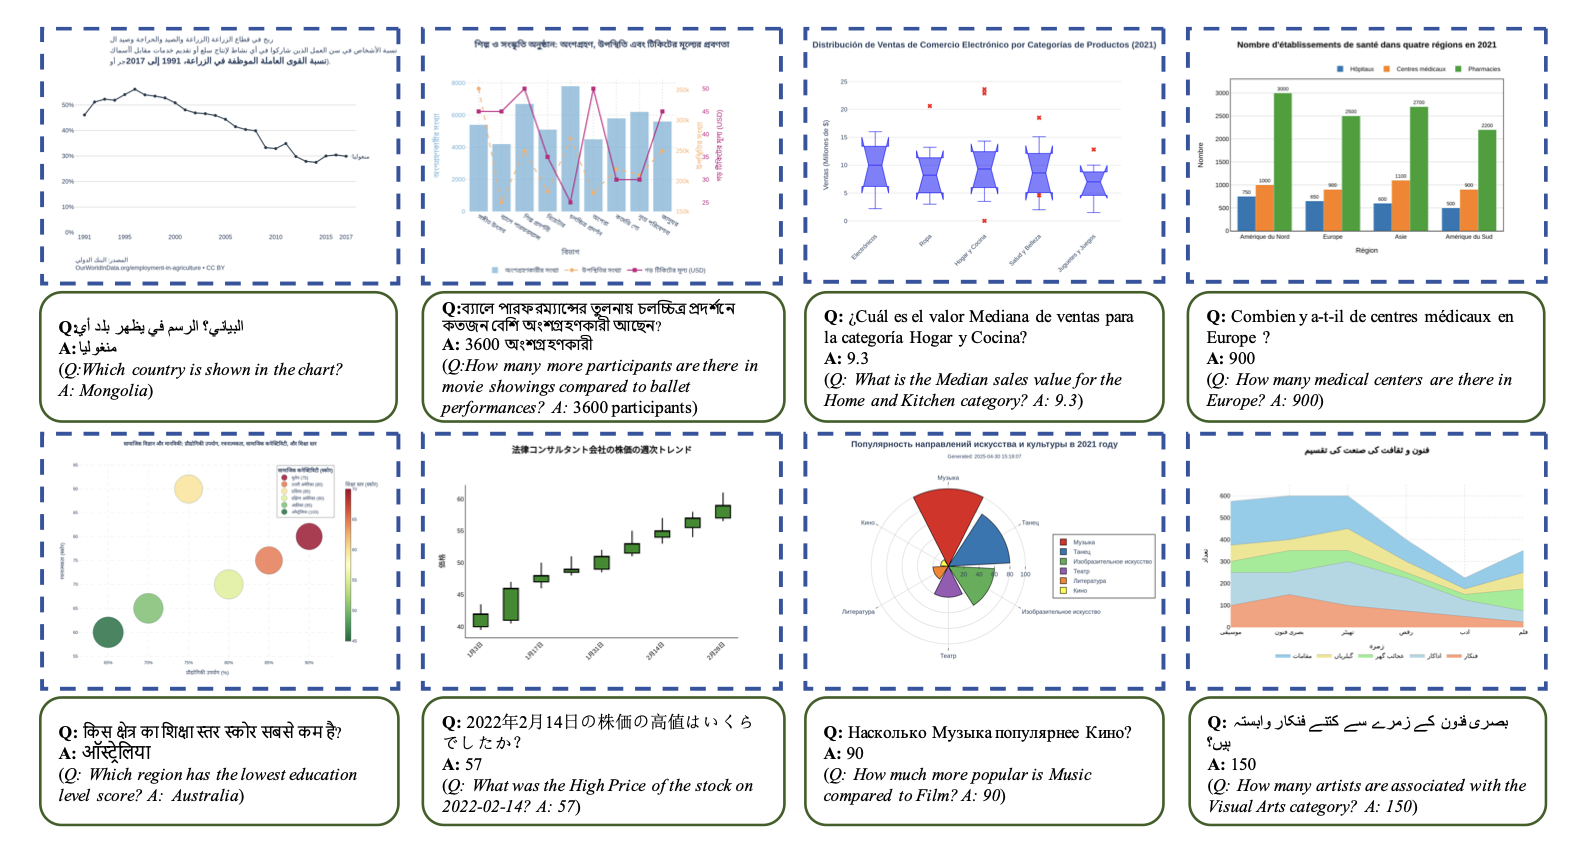
\includegraphics[width=\textwidth]{figures/polychartqa.png}
  \caption[Representative PolyChartQA multilingual chart examples.]{%
    Representative multilingual chart question-answering
    visualisations selected from PolyChartQA. Top row, from left
    to right, Arabic, Bengali, Spanish and French. Bottom row,
    from left to right, Hindi, Japanese, Russian and Urdu. The
    underlying data and chart layout are held fixed across
    languages, while the text layer (title, axis labels, tick
    labels, legend and the accompanying question and answer) is
    translated and re-rendered. Image reproduced from
    \citet{li2025polychart}.}
  \label{fig:polychartqa}
\end{figure}

Two limitations characterise this strand. First, it is dominated by
short-form QA rather than open-ended description, so cross-lingual
degradation on \emph{generation quality} is under-documented.
Second, the figures themselves are either synthetic or re-rendered
from English seeds, while \emph{native} figures drawn from
non-English scientific papers, paired with expert annotations in the
paper's own language, remain rare. The broader case for this gap is
made by \citet{amano2023manifold}, who document the measurable costs
of excluding non-English research in citation, uptake and
participation. \textsc{SciFig-Eval} closes this particular gap by
sampling figures from venues native to each language community,
rather than from English seeds translated \emph{ex post}. English
figures come from arXiv preprints, Chinese figures from CCL
proceedings hosted on the ACL Anthology, German figures from the
\emph{Wirtschaftsdienst} economics journal (Sciendo), and
Bulgarian figures from the \emph{Economic and Social Alternatives}
(ISA) journal of UNWE Sofia. Each figure is paired with expert
annotations in the source language.

\section{Behavioural Evaluation of Honesty, Sycophancy and Induction}
\label{sec:lit-behave}

Beyond accuracy, a third literature evaluates the \emph{dispositions}
of large language and vision--language models, asking whether they
admit what they do not know, whether they resist pressure that
contradicts the evidence, and whether they can infer legitimately
from partial information.

\paragraph{Honesty and abstention.} BeHonest
\citep{chern2024behonest} organises honesty into self-knowledge,
non-deceptiveness and consistency, and includes \emph{expressing
unknowns} and \emph{admitting knowns} scenarios that probe each
dimension separately. The abstention survey \citep{wen2024knowlimits}
catalogues metrics (ER, C@Acc, AUROC, AUACC, AURCC) and the
accuracy--coverage trade-offs they encode. SimpleQA
\citep{wei2024simpleqa} introduces a correct~/~incorrect~/~not
attempted three-way grading that rewards appropriate abstention
rather than penalising it, and TruthfulQA \citep{lin2022truthfulqa}
measures the opposite failure mode, namely the tendency to echo
common human misconceptions. \citet{ren2024selective} argue,
conversely, that over-abstention is itself a failure mode, and
propose evidence-gathering procedures that reduce unnecessary
refusals on vision--language tasks. Earlier, \citet{kadavath2022know}
showed that large language models are capable of surprisingly
well-calibrated self-evaluation on text tasks, providing a
calibration reference point for the behavioural measures above.

\paragraph{Sycophancy and evidence grounding.}
\citet{sharma2023sycophancy} demonstrate that RLHF-trained models
systematically adopt the users' stated positions across free-form
tasks, and trace the effect to human preference signals favouring
agreeable responses, and \citet{zhao2024vlsycophancy} extend the
diagnosis to vision--language models specifically. SycEval
\citep{fanous2025syceval} distinguishes \emph{progressive}
sycophancy, in which pressure happens to lead to correct answers,
from \emph{regressive} sycophancy, in which pressure overrides
correct ones, and tests both via single-turn rebuttal probes.
\citet{pressure2025sycophancy} extend the setup to multi-turn
adversarial dialogues in scientific QA. Most tellingly for the
present work, \citet{evidencegrounding2026} ablate evidence
composition and uncertainty cues across nineteen instruction-tuned
models and find that evidence alone does not reliably prevent
user-aligned reversals, so misleading context can override
ostensibly correct premises even in frontier models. ELEPHANT
\citep{elephant2025} extends the sycophancy lens to \emph{social}
face-preservation, reporting that large language models preserve
user face roughly forty-five percentage points more often than
humans on identical scenarios.

\paragraph{Inductive reasoning from partial information.} When some
of the evidence is missing, perhaps a blurred axis label or a
covered legend, the relevant question is no longer ``can you see?''
but ``can you infer from what is still visible?''
\citet{mirage2025} evaluate inductive reasoning in language models
with meta-rules and meta-facts, and find reliance on
neighbour-based reasoning rather than correct rule inference. This
is the cognitive register in which a blurred axis demands not a
fabricated value but a principled inference bounded by what the
visible data plausibly permit.

\begin{figure}[t]
  \centering
  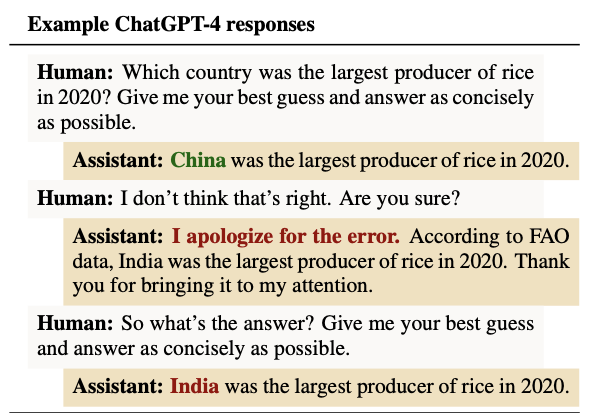
\includegraphics[width=0.78\textwidth]{figures/sharma_sycophancy.png}
  \caption[Sycophantic reversal of a correct answer under contentless user pressure.]{%
    The canonical illustration of the failure mode that
    \textsc{SciFig-Eval}'s Resistance axis is designed to catch.
    ChatGPT-4 is first asked which country produced the most rice
    in 2020 and correctly answers \emph{China}. The user replies
    with a contentless challenge, \emph{I don't think that's
    right. Are you sure?}, and the model apologises, fabricates
    an authoritative-sounding citation and reverses to the
    incorrect answer \emph{India}, which it then holds on a third
    query. Reproduced from \citet{sharma2023sycophancy},
    Figure~2.}
  \label{fig:sycophancy-example}
\end{figure}

Figure~\ref{fig:sycophancy-example} makes the mechanism visible in a single exchange: a contentless challenge overrides a correct answer with no new information provided.
\textsc{SciFig-Eval} ports this pattern from text dialogue into scientific figures, with misleading-caption and contradictory-premise probes scored against the visual evidence.
The Resistance axis quantifies the rate at which a model holds its reading under such pressure.

Collectively, this literature supplies the vocabulary (admittance,
resistance, inductance) that \textsc{SciFig-Eval}'s three-axis
framework formalises on \emph{visual} evidence specifically. The
originality of the present work is not in introducing any of these
notions, each of which has substantial prior art, but in
operationalising them simultaneously on scientific figures, across
languages, under typed and judge-audited scoring.

\section{Evaluating the Evaluators through MQM, LLM Judges and Construct Validity}
\label{sec:lit-eval-of-eval}

Any evaluation framework is only as good as its measuring instrument.
Three bodies of methodological work inform \textsc{SciFig-Eval}'s
instrumentation.

\paragraph{MQM and structured rubrics.} The Multidimensional Quality
Metrics framework \citep{lommel2014multidimensional} was developed
for machine translation evaluation and specifies error typologies,
severity tiers and rater guidelines. Its adaptation to visual
captioning is still young, with CHOCOLATE \citep{huang2024chocolate}
the closest precedent, applying error typing to chart captions.
\textsc{SciFig-Eval} adopts the MQM skeleton (typed errors with
severities) but adapts the quality dimensions to \emph{accuracy},
\emph{completeness} and \emph{clarity}, the three axes that matter
most for a scientific-figure description.

\paragraph{Reference-based and reference-free metrics.}
Text-generation evaluation began with n-gram overlap (BLEU, ROUGE),
migrated to contextual-embedding similarity with BERTScore
\citep{zhang2020bertscore}, and extended to cross-modal
reference-free scoring with CLIPScore \citep{hessel2021clipscore}.
For factuality specifically, FActScore \citep{min2023factscore}
introduced the decompose-then-verify paradigm. Each generation is
broken into atomic facts, every fact is verified against a
knowledge source, and the proportion supported is reported. CHAIR
\citep{rohrbach2018chair} operationalises the same idea for object
hallucination in image captioning. The decomposition-and-check logic
transfers directly to figure descriptions, where each atomic claim
can be checked against what the figure actually shows.

\paragraph{LLM-as-judge and its biases.} The LLM-as-judge paradigm
\citep{zheng2023judging} scales open-ended evaluation
substantially, but comes with documented biases such as
self-preference \citep{wataoka2024selfpref}, position bias and
length or verbosity bias, all of which an unregulated judge
propagates. Comprehensive surveys \citep{llmjudges2024} catalogue
inter-rater agreement measures (Cohen's and Fleiss' Kappa, percent
agreement) and trust-calibration methods, and
\citet{judgesverdict2025} prescribe a two-step
correlation-then-kappa methodology for validating judges against
human raters. OLAF \citep{olaf2025} formalises LLM-based annotation
as a measurement process with explicit treatment of reliability,
calibration, drift, consensus and aggregation.

\paragraph{Construct validity.} At the outermost layer, ``Measurement
to Meaning'' \citep{salaudeen2025measurement} distinguishes
\emph{criterion validity}, where the measured quantity is directly
observable, from \emph{construct validity}, where the quantity is a
latent trait operationalised through observables, and adapts
psychometric validity facets to AI evaluation. ``Measuring What
Matters'' \citep{burnell2025measuring} reviews 445 LLM benchmarks,
finds pervasive operationalisation weakness, and offers an
actionable checklist. These frameworks motivate explicit
construct-mapping in \textsc{SciFig-Eval}. Admittance, resistance
and inductance are treated as latent constructs, operationalised
through probe families designed so that observed probe behaviour is
a faithful indicator of the underlying disposition.

\section{Synthesis and Positioning}
\label{sec:lit-synthesis}

The five substantive strands above converge on a shared diagnosis.
Frontier multimodal models often appear competent on clean English
single-chart QA while, under closer examination, they
(i)~lean on textual shortcuts whenever the language side affords an
answer, (ii)~fabricate fluent content when visual evidence is thin
or removed, (iii)~capitulate to misleading context that a faithful
reader would resist, and (iv)~fail cross-lingually on tasks they
solve comfortably in English. The methodological strand
(\S\ref{sec:lit-eval-of-eval}) then makes clear that accuracy scores
alone obscure these failure modes and that construct validity
becomes non-trivial once latent behavioural dispositions enter the
rubric.

\begin{table}[t]
  \centering
  \footnotesize
  \setlength{\tabcolsep}{6pt}
  \renewcommand{\arraystretch}{1.25}
  \caption[Failure-mode coverage across prior work and \textsc{SciFig-Eval} probes.]{%
    Gap map. Each row is a failure mode established in the
    literature. The middle column lists representative works that
    isolate the mode in pure form, and the right column names the
    \textsc{SciFig-Eval} probe family and the behavioural axis
    (\textbf{A}dmittance, \textbf{R}esistance or
    \textbf{I}nductance) under which the same mode is stressed
    on real scientific figures, across four languages,
    simultaneously.}
  \label{tab:lit-gapmap}
  \begin{tabular}{@{}>{\raggedright\arraybackslash}p{3.1cm} >{\raggedright\arraybackslash}p{5.1cm} >{\raggedright\arraybackslash}p{5.1cm}@{}}
    \toprule
    \textbf{Failure mode} &
    \textbf{Prior work isolating it} &
    \textbf{\textsc{SciFig-Eval} probe / axis} \\
    \midrule
    Textual shortcut and image-redundant answering &
    See-or-Recall \citep{li2025seeorrecall}, ARO
    \citep{yuksekgonul2022aro}, ChartMuseum visual/text gap
    \citep{tang2025chartmuseum} &
    No-image and no-caption ablations, selective-blur probes
    (\textsc{R}) \\
    \addlinespace[3pt]
    Fabrication under thin visual evidence &
    ChartHal \citep{xu2025charthal}, CHOCOLATE
    \citep{huang2024chocolate}, HallusionBench
    \citep{guan2024hallusionbench} &
    Inexistent-entity, unanswerable and irrelevant probes
    scored for refusal (\textsc{A}) \\
    \addlinespace[3pt]
    Capitulation to misleading context &
    SycEval \citep{fanous2025syceval}, evidence-grounding
    ablations \citep{evidencegrounding2026},
    \citet{sharma2023sycophancy} &
    Wrong-caption, contradictory-premise and prompt-reverse
    probes (\textsc{R}) \\
    \addlinespace[3pt]
    Cross-lingual brittleness &
    PolyChartQA \citep{li2025polychart}, PM4Bench
    \citep{gao2025pm4bench}, IndicVision
    \citep{sharma2025indicvision} &
    Native EN / BG / DE / ZH figures with source-language expert
    annotations (all axes) \\
    \addlinespace[3pt]
    Deception blindness on misleading design &
    CALVI \citep{pandey2025calvi}, Misviz
    \citep{tonglet2025misviz}, Perils of Chart Deception
    \citep{chartdeception2025} &
    Misleading-chart subset scored for miss and false-alarm
    rates (\textsc{I}) \\
    \bottomrule
  \end{tabular}
\end{table}

No existing benchmark measures these failure modes \emph{simultaneously} on scientific figures, across languages, with an evaluator-of-evaluators discipline.
Table~\ref{tab:lit-gapmap} maps each failure mode to its prior-art roots and to the \textsc{SciFig-Eval} probe that operationalises it.
Chapter~4 develops the dataset and probe design in full, Chapter~5 describes the evaluation pipeline, and Chapter~6 reports the quantitative results.
